\documentclass[a4paper,12pt]{report}
    \title{Service Registry}
\author{Theodor Bogdan Vr\^ancean}
\date {Iunie 2018}

\usepackage[romanian]{babel}

\usepackage{graphicx}
\graphicspath{{"./Images/"}}

\usepackage[
    backend=biber,
    style=verbose,
    sorting=ynt
]{biblatex}
\addbibresource{References.bib}

\begin{document}
\maketitle
\tableofcontents
\chapter{Introducere}
\section{Arhitectura de microservicii}

Arhitectura de microservicii este o abrodare relativ nou\u a \^ in dezvoltarea de software.
Microserviciile reprezint\u a aplica\c tii mici \c si autonome care lucreaz\u a \^ impreun\u a
\footcite{buildingMicroservices1}. Ele sunt considerate mici relativ la un sistem monolitic care ar
oferi toate func\c tionalit\u a\c tiile de care aplica\c tia are nevoie.Cu toate acestea un mictoserviciu poate oferi orice
fel de func\c tionalit\u a\c ti,incep\^and cu ceva simplu precum desc\u arcarea de fi\c siere, p\^an\u a la
complexe precum analizarea imaginilor.
Aceast\u a aboradare arhitecturala a venit ca o alternativ\u a la arhitectura monolitic\u a, \^in care exist\u a
un singur server care satisface toate necesit\u a\c tile unei aplica\c tii.Limit\u arile acestei abord\u ari ies la iveal\u a
odat\u a cu cre\c sterea aplica\c tiei.
Pentru a \^intelege de ce arhitectura  de microservicii \^incepe sa \^inlocuiasc\u a arhitectura monolitic\u a
trebuie sa cunoa\c stem urm\u atoarele beneficii:
\begin{itemize}
	\item Din cauza dimensiunii \c si complexit\u a\c tii unui proiect monolitic,
	      acesta este dificil de in\c teles \c ,motiv pentru care schimb\u arile sunt mai dificil de facut \c si exist\u a
	      un risc mai mare ca acestea s\u a produc\u a efecte nedorite.Aceste probleme pot fi atenuate printr-un
	      cod de calitate dar acest lucru se \^ inatmpla de prea pu\c tine ori. Schimb\u arile aduse unui microserviciu nu afecteaz\u a alte
	      module \c si datorit\u a dimensiunii reduse a acestora, ele sunt \c si mai u\c sor de \^inteles pentru programtori, astfel
	      scade probabilitatea erorilor.Se poate spune ca microserviciile duc un pas mai departe principiul singurei responsabilit\u a\c ti,
	      definit de Robert C. Martin.
	\item Pentru dezvoltarea unei aplica\c tii monolitice trebuie sa alegem tehnologii standardizate care s\u a poata
	      realiza toate cerin\c tele aplica\c tiei. Pe de alta parte,daca avem mai multe microservicii care colaboreaz\u a nu exist\u a
	      aceast\u a limitare,ceea ne permite s\u a alegem unealta cea mai portivit\u a pentru fiecare serviciu.
	      S\u a lu\u am spre exemplu un site al unei pizzerii care folose\c ste microservicii (Fig 1).
	      Partea de front-end doar apeleaz\u a serviciile c\^and are nevoie.Putem avea un server scris
	      in C\# care folose\c ste un sistem de gestiune a bazei de date Microsoft Sql Server,
	      unul scris \^in php cu MySql \c si unul scris in Node.js cu mongoDb \ref{fig:PizzaMicroservicii}.Deoarce toate comunic\u a prin
	      protocolul http ,acestea pot lucra \^impreun\u a,fiecare av\^and responsabilitatea sa.
	      \begin{figure}[!htb]
		      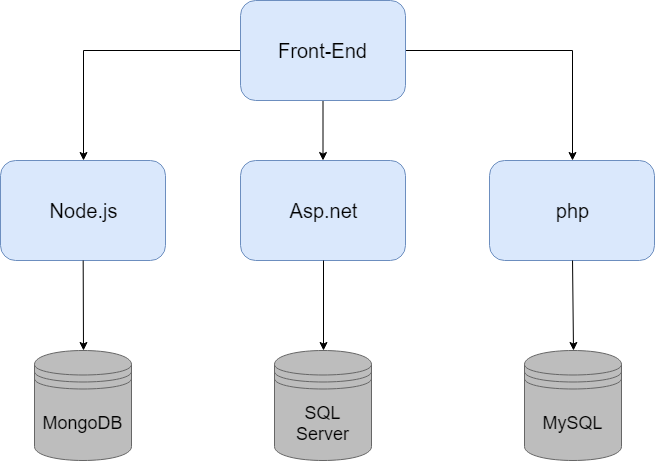
\includegraphics[width=\textwidth,keepaspectratio]{PizzaMicroservicii}
		      \caption{Arhitectur\u a cu microservicii pentru un site de pizzerie}
		      \label{fig:PizzaMicroservicii}
	      \end{figure}
	\item O aplica\c tie a c\u arei componente sunt distribuite este mai rezistent\u a, \^in sensul c\u a dac\u a un
	      serviciu este compromis, func\c tionalita\c tile care nu depind de acel serviciu vor continua s\u a func\c tioneze.
	      \^In cazul unei aplica\c tii clasice, tot sistemul va fi compromis din cauza unei singure componente.
	\item Cu un serviciu mare,monolitic, trebuie sa scal\u am totul \^imreun\u a.O parte mic\u a
	      a \^intregului nostru sistem, este constr\^ans\u a \^in performan\c t\u a, dar dac\u a
	      acest comportament este blocat \^intr-o aplica\c tie monolitic\u a gigant\u a, trebuie sa scal\u am totul \^impreun\u a
	      ca o bucat\u a \footcite{buildingMicroservices5}.Acest lucru se face deobicei folosind mai multe servere
	      \c si un server de tip load balancer care s\u a distribuie cererile c\u atre unul din acele servere pentru
	      a reduce munca depus\u a de un singur server o depune, astfel evit\^and supra\^incarcarea si cresc\^and performan\c ta.
	      \^In cazul arhitecturii cu microservicii, ajunge s\u a scalam doar acele servicii care au probleme de performan\c ta.
	\item Microserviciile ofer\u a \c si reutilizabiliate, ele pot fi utilizate de multiple aplica\c tii.
		  Daca dou\u a aplica\c tii au func\c tionalita\c ti similare, acestea nu trebuie implementate de dou\u a ori, aceast\u a func\c tionalitate
		  poate fi oferit\u a de un serviciu comun , folosit de ambele aplica\c tii.Uneori acest lucru este chiar necesar, dac\u a un produc\u ator de software
		  are mai multe aplica\c tii ce necesit\u a autentificare, este mult mai comod pentru utilizator s\u a aib\u a un singur cont cu care s\u a se autentifice in fiecare aplica\c tie 
		  \c si acest lucru este avantajos si pentru produc\u ator.
		  Microserviciile pot fi f\u acute \c si publice, pe baza unei chei de autentificare,pe care le pot folosi pentru aplica\c tiile lor,persoane in afara companiei produc\u atoare.
		  \^In prezent exist\u a multe servicii de meteorologie, gratuite sau contra cost, pe care le putem folosi \^in aplica\c tiile noastre.
\end{itemize}

Bine\^in\c teles arhitectura cu microservicii nu este o solu\c tie miraculoas\u a la toate problemele,
adat\u a cu aceste beneficii, ea vine \c si cu dezavantajele.Fiind un sistem distribuit toate
problemele acestor sisteme afecteaz\u a si microservicii.
O problem\u a este men\c tinerea leg\u aturii \^intre componentele aplica\c tiei.Un serviciu \^isi poate schimba 
adresa,poate deveni inactiv sau poate fi \^inlocuit.\^In aceste situa\c tii se va pierde func\c tionalitatea pe care acesta o 
ofer\u a.Pentru a remedia aceast\u a situa\c tie ar trebui sa schimb\u am adresele la care aplica\c tia se a\c steapt\u a sa 
gaseasc\u a serviciul respectiv, dup\u a care ar trebui sa to\c ti utilizatorii sa sa fac\u a un update la noua versiune.
Aceast\u a solu\c tie simpl\u a nu doar c\u a nu este convenabil\u a ,dar devine imposibil\u a dac\u a avem servicii care ruleaz\u a 
pe ma\c sini virtuale sau containere de docker care suntcreate dinamic \^in func\c tie de nevoie.
Solu\c tia pe care eu am implementat-o este un sistem de tip service registry.
Acesta este la baz\u a un serviciu web care face leg\u atura \^intre microservicii.Astfel aplica\c tia \c si serviciile trebuie 
s\u a cunoasc\u a doar serviciul de \^inregistrare si el se va furniza datele despre celelalte servicii necesare func\c tionarii aplica\c tiei. 
Serverul de \^ inregistrare ofer\u a trei opera\c tii de baza:
\begin{enumerate}
	\item \textbf{\^Inregistrarea}
	
			Serviciile se pot \^inregistra la server atunci c\^and \^i\c si \^incep func\c tionarea.
			\^In cazul \^in care serviciu folosit este facut de un alt produc\u ator care nu cunoa\c ste acest 
			mecanism sau nu este dispus s\u a \^il foloseasc\u a,exist\u a \c si posibilitatea ca administratorul 
			aplica\c tiei sa \^inregistreze serviciul respectiv manual prin intermediul intefer\c tei grafice.
	\item \textbf{De\^inregistrarea}

		  Serviciile au posibilitatea de a se de\^inregistra,acest lucru ar trebuie s\u a fie f\u acut la \^inchiderea 
		  serviciului.\^In cazul in care acestea devin inactive far\u a a se de\^inregistra, serverul le va de\^inregistra
		  automat.
	\item \textbf{C\u autarea}

		  Aplica\c tia \c si microserviciile pot c\u auta un serviciu \^inregistrat \^in server.
\end{enumerate}	
\chapter{Tehnologii}

C\# este un limbaj de programare. \^ s \c t \^a

\section{.Net Framework}
\section{Entity Framework}
EntityFramework este un ORM(Object Relational Mapper) open-source pentru platforma .Net.
\section{Asp.Net}
\section{MVC pattern}
\section{Microsoft Sql Server}

\chapter{Utilizare}

\end{document}
